\chapter{Results}
{\label{ch:results}}

\section{Results and Discussion}
This section details the empirical findings obtained from evaluating the Legal Precedent Assistant framework outlined in IEEE\_LPA\_Paper (1).pdf. The evaluation is structured across three primary phases: vector database generation performance, domain-adaptive pre-training (DAPT) token metrics, and task-specific supervised fine-tuning accuracies for legal judgment pipeline operations.

\subsection{Vector Database and Embedding Generation Performance}
The ingestion pipeline processed a curated historical dataset to construct a highly optimized hybrid semantic index. The structural breakdown and performance benchmarks of the data pipeline are summarized below:

\begin{itemize}
	\item \textbf{Source Corpus Capacity:} The system successfully extracted, cleaned, and compiled 26,515 distinct Supreme Court case records spanning from 1990 to 2025.
	\item \textbf{Text Chunk Segmentation:} To preserve local statutory contexts and overcome encoder length limitations, the raw text was partitioned using a recursive splitting mechanism. The operation maps each document into a sequence of smaller chunks:
	\begin{equation}
		C=\{c_{1},c_{2},...,c_{n}\} \text{}
	\end{equation}
	Each text chunk $c_i$ was limited to a maximum length of 1,500 characters with a sliding window overlap of 200 characters to prevent context truncation at boundaries. This generated an expanded target corpus containing 737,116 discrete text chunks.
	\item \textbf{Hardware-Accelerated Vectorization:} Using the \texttt{BAAI/bge-small-en-v1.5} sentence transformer model, textual data was mapped into low-dimensional dense representations:
	\begin{equation}
		v_{i}=f_{BGE}(c_{i}), \quad v_{i}\in\mathbb{R}^{384} \text{}
	\end{equation}
	\item \textbf{Execution Throughput:} Distributing the processing workloads across a multi-process pool utilizing dual NVIDIA Tesla T4 GPUs with an optimized evaluation batch size of 64, the pipeline completed vector generation for all 737,116 chunks in 58.75 minutes.
\end{itemize}
The resulting arrays were serialized into a multi-device payload (\texttt{sc\_vectors.npy} and \texttt{sc\_payload.json}) and successfully ingested into Chroma DB alongside normalized string arrays containing categorical legal metadata keys.

\subsection{Domain-Adaptive Pre-Training (DAPT) Evaluation}
Unsupervised domain-adaptive pre-training (DAPT) was executed to adapt general-domain foundational encoders and parameterized large language models (LLMs) to the complex linguistic realities of the Indian legal lexicon. The models were evaluated using cross-entropy token validation loss and vocabulary perplexity under a strict head-tail tokenization strategy to handle hardware constraints.

\begin{table}[htbp]
	\caption{DAPT Perplexity and Loss Across Evaluated Models}
	\label{tab:dapt_metrics}
	\centering
	\begin{tabular}{|l|c|c|c|c|}
		\hline
		\textbf{Model} & \textbf{Epochs} & \textbf{Perplexity} & \textbf{Validation Loss} & \textbf{Batch Size} \\ \hline
		BERT-small & 2 & 8.80 & 2.1746 & 8 \\ \hline
		BERT-medium & 2 & 7.99 & 2.0783 & 4 \\ \hline
		LegalBERT-uncased & 2 & 6.63 & 1.8922 & 4 \\ \hline
		IN-LegalBERT & 2 & 5.12 & 1.6374 & 4 \\ \hline
		Llama 3.1 8B & 1 & 3.00 & 1.7200 & 2 \\ \hline
		DeepSeek R1 8B & 1 & 2.60 & 1.6500 & 1 \\ \hline
	\end{tabular}
\end{table}

\subsubsection{Analysis of DAPT Gains}
\begin{itemize}
	\item \textbf{Baseline vs. Adapted Encoders:} Baseline models like BERT-small and BERT-medium, originally trained on generic corpora, initially lacked the specialized vocabulary necessary for dense legal terminology, yielding higher perplexity scores. Conversely, models with pre-existing legal baselines (e.g., LegalBERT-uncased) adapted more efficiently. IN-LegalBERT achieved the lowest perplexity among encoders (5.12) and a loss of 1.6374, proving that adapting existing legal baselines directly to Indian judicial contexts significantly refines vocabulary distribution.
	\item \textbf{Large Language Model Scaling:} Parameterized architectures including Llama 3.1 8B and DeepSeek R1 8B demonstrated exceptional zero-to-one shot adaptation capability. DeepSeek R1 8B reached an ultra-low vocabulary perplexity of 2.60 within a single training epoch.
	\item \textbf{Overfitting Mitigation:} Over prolonged runs, models tended to memorize exact statutory phrases or specific Indian Penal Code (IPC) combinations rather than generalizable semantic boundaries. Implementing a validation-driven early stopping strategy restricted training to 1--2 epochs for larger models and 2--3 epochs for smaller models, effectively arresting performance degradation.
\end{itemize}





\subsection{Downstream Supervised Fine-Tuning Performance}
Following DAPT, task-specific supervised fine-tuning was executed to calibrate both encoder architectures and generative large language models (LLMs) for localized pipeline operations, specifically Layer 1 (IPC/BNS mapping), Layer 2 (evidence consistency auditing), and Layer 4 (verdict prediction). 

To manage severe class imbalances across statutory labels, encoder models utilized an optimized processing window and focal loss ($\alpha=0.25, \gamma=2.0$). Conversely, the parameterized LLMs (Llama and DeepSeek variants) were fine-tuned utilizing Quantized Low-Rank Adaptation (QLoRA) in 4-bit Normal Float (nf4) precision, leveraging an expanded 2048-token context window to process complex, multi-span legal reasoning.


\begin{table}[htbp]
	\caption{Supervised Fine-Tuning Operational Metrics}
	\label{tab:finetuning_metrics}
	\centering
	\begin{tabular}{|l|c|c|c|c|}
		\hline
		\textbf{Model} & \textbf{Epochs} & \textbf{Validation Accuracy} & \textbf{$\text{F}_1$ Score} & \textbf{Validation Loss} \\ \hline
		BERT-small & 3 & 67\% & 0.65 & 0.6517 \\ \hline
		BERT-medium & 3 & 71\% & 0.69 & 0.0351 \\ \hline
		LegalBERT-uncased & 3 & 78\% & 0.76 & 0.0311 \\ \hline
		IN-LegalBERT & 3 & 85\% & 0.84 & 0.0250 \\ \hline
		Llama-3.1-3B                & 3 & 86\% & 0.85 & 0.0215 \\ \hline
		Llama-3.1-8B                & 3 & 88\% & 0.87 & 0.0188 \\ \hline
		DeepSeek-R1-Distill-8B & 3 & 90\% & 0.89 & 0.0142 \\ \hline
	\end{tabular}
\end{table}

\subsubsection{Key Performance Discoveries}
\begin{itemize}
	\item \textbf{Downstream Accuracy Breakthrough:} General-domain models (BERT-small and BERT-medium) converged steadily but displayed a capped semantic capacity, achieving modest validation accuracies of 67\% and 71\%. Deepseek R1 Distill 8B leveraged international domain knowledge \& reasoning capabilities to achieve 78\% accuracy.
	\item \textbf{Optimized Domain Leadership:} The domain-adapted Deepseek R1 model significantly outperformed all other encoder architectures, reaching a peak validation accuracy of 90\% and a top $\text{F}_1$ score of 0.89, alongside a minimal validation loss of 0.0142. These results demonstrate that combining DAPT over localized Indian legal data with targeted supervised fine-tuning drastically improves model sensitivity toward case citation structures, statutory configurations, and factual patterns.
\end{itemize}


\subsubsection{Analysis of Fine-Tuning Performance}
The empirical results compiled in Table~\ref{tab:finetuning_metrics} reveal a clear performance scaling trajectory correlated with model parameter size and specialized domain exposure:
\begin{itemize}
	\item \textbf{Encoder Limitations vs. Adaptation:} Generic encoders (BERT-small and BERT-medium) exhibited constrained semantic capacity, capping accuracy at 67\% and 71\% respectively. While domain adaptation allowed \texttt{Deepseek R1} to achieve a highly competitive 90\% accuracy among encoder-only frameworks, it was systematically outpaced by LLMs capable of broader contextual comprehension such as Gemini.
	\item \textbf{Generative LLM Dominance via QLoRA:} Parameter-efficient fine-tuning via QLoRA yielded immediate performance breakthroughs. Llama-3.1-3B, Llama-3.1-8B and Deepseek R1 Distill 8B achieved validation accuracies of 86\% and 88\% 90\% respectively. 
	\item \textbf{Peak Fine-Tuned Performance:} The \texttt{DeepSeek-R1-Distill-8B} model established the highest fine-tuned baseline, achieving an \textbf{accuracy of 90\%}, an \text{F}$_1$ score of 0.89, and a minimal validation loss of 0.0142. This demonstrates that integrating structured reasoning tokens during distillation significantly boosts a model's aptitude for evaluating evidence contradictions and parsing intricate judicial logic.
\end{itemize}

\subsection{Proprietary API Integration and Benchmark Evaluation}
As noted in Section I, powerful commercial large language models—specifically Google Gemini, OpenAI ChatGPT, and Anthropic Claude—possess immense context windows and massive parameter counts that cannot be replicated or locally fine-tuned within consumer-tier hardware environments. Consequently, these models were omitted from the supervised fine-tuning environment matrix (Table~\ref{tab:finetuning_metrics}) and were instead evaluated via zero-shot and few-shot API integrations using a pipeline routing framework.

\subsubsection{Gemini API Empirical Insights}
Despite lacking targeted local fine-tuning on the custom Indian Legal Corpus, the \textbf{Gemini API integration emerged as the absolute best overall performer across the end-to-end framework}. This exceptional out-of-the-box performance is attributed to two structural factors:
\begin{enumerate}
	\item \textbf{Context Window Architecture:} The massive context window offered by the Gemini API easily ingested entire multi-page Supreme Court judgments without requiring severe head-tail truncation strategies or strict token limits. This allowed the model to maintain complete, uninterrupted structural links between early trial arguments and final settlement orders.
	\item \textbf{Advanced Multilingual Parsing:} Gemini demonstrated superior linguistic resilience when handling regional vernacular inputs (such as Marathi and Hindi court summaries). Where smaller local models failed due to poorly translated legal jargon, Gemini's cross-lingual reasoning capacity smoothly bypassed extraction bottlenecks, producing highly coherent abstractive summaries under the 150-word cap.
\end{enumerate}

\subsection{End-to-End Modular Pipeline Verification}
Operational tracking of cases moving through the six-layer architecture verified the technical execution of individual modules as intended by the framework design:

\subsubsection{Document Extraction and Fact Synthesis (Layers 0 \& 1)}
The parallelized PyMuPDF extraction successfully ingested complex multi-page files, retaining structural anchors like ``Arguments'' and ``Issues'' while purging footer noise. For named entity recognition (NER) and statutory mapping, heuristic regular expressions were used. Preamble variables (judges, party names, locations) and applicable statutory sections were extracted to build the core context for downstream tracking.

\subsubsection{Evidence Scrutinization and Audit (Layer 2)}
Using 4-bit precision LoRA adapters, the parameterized models executed deep consistency audits across opposing affidavits and historical records. Because the context lengths were expanded to 2048 tokens via QLoRA, the system successfully audited cross-document statements (comparing First Information Reports (FIRs), Evidence Affidavits, Petitions/Responses, and Domestic Incident Reports (DIRs)), identifying factual contradictions and assigning structured truth scores to target evidence payloads.

\subsubsection{Sub-Space Precedent Retrieval (Layer 3)}
When presented with a case scenario vector $q$, Chroma DB bypassed open-ended searches by implementing hard metadata filters based on the extracted statutory codes. Once categorized sub-spaces were isolated, the system measured directional distances using the Cosine Similarity metric:
\begin{equation}
	Sim(q,v_{i})=\frac{q\cdot v_{i}}{||q||||v_{i}||}=\frac{\sum_{k=1}^{384}q_{k}v_{ik}}{\sqrt{\sum_{k=1}^{384}q_{k}^{2}}\sqrt{\sum_{k=1}^{384}v_{ik}^{2}}} \text{}
\end{equation}
The system consistently isolated the top-$k$ mathematically closest text chunks, minimizing hallucination vectors by injecting verified factual precedents directly into the prediction prompt.

\subsubsection{Verdict Prediction and Summarization (Layers 4 \& 5)}
By synthesizing the contextual outputs from the previous phases (extracted mappings, truth scores, and retrieved precedents), the pipeline effectively generated concise trial outcomes and verdict sentences. In the final phase, abstractive summarization models stripped away complex legalese to condense multi-page judicial proceedings into clear, public-comprehensible case outlines bounded strictly under the target threshold of 150 words.

\subsection{Performance Trade-Offs and Pipeline Constraints}
Despite reaching a high benchmark accuracy of 85\%, empirical monitoring identified clear operational boundaries within the current deployment:

\begin{itemize}
	\item \textbf{Token-Length and GPU Bottlenecks:} Local hardware configurations (4GB VRAM constraints on the local NVIDIA GTX 1650) forced a tight 128-token limit during encoder training. While the head-tail tokenization strategy successfully captured introductory facts and final judgments, it omitted intermediate text blocks, limiting the model's ability to map long-range contextual arguments found in massive files.
	\item \textbf{Indic Language Degradation:} The pipeline includes translation tools to parse regional vernacular case documents written in Marathi or Hindi. However, due to a severe shortage of specialized, domain-trained Indic translation models, legal jargon frequently suffered from poor translation quality, causing downstream drops in predictive precision and summary completeness.
	\item \textbf{Statutory Rule Over-reliance:} The extraction of specific sections relies heavily on regular expressions and general-purpose NER blocks, which occasionally misclassified or skipped highly complex or nested cross-statute references within complex complaints.
\end{itemize}





\subsection{System Interface and Interaction Results}
\label{sec:streamlit_gemini_ui}

The system features a Streamlit-based web interface designed to streamline the document analysis workflow for legal professionals. Below Figures demonstrate the end-to-end process: from the initial document upload and parsing to the final generation of a simplified, jargon-free summary provided via PymMuPDF(Fitz), NLLB, Chroma DB and Gemini API.

\begin{figure}[htbp]
	\centering
	\captionsetup{justification=centering}
	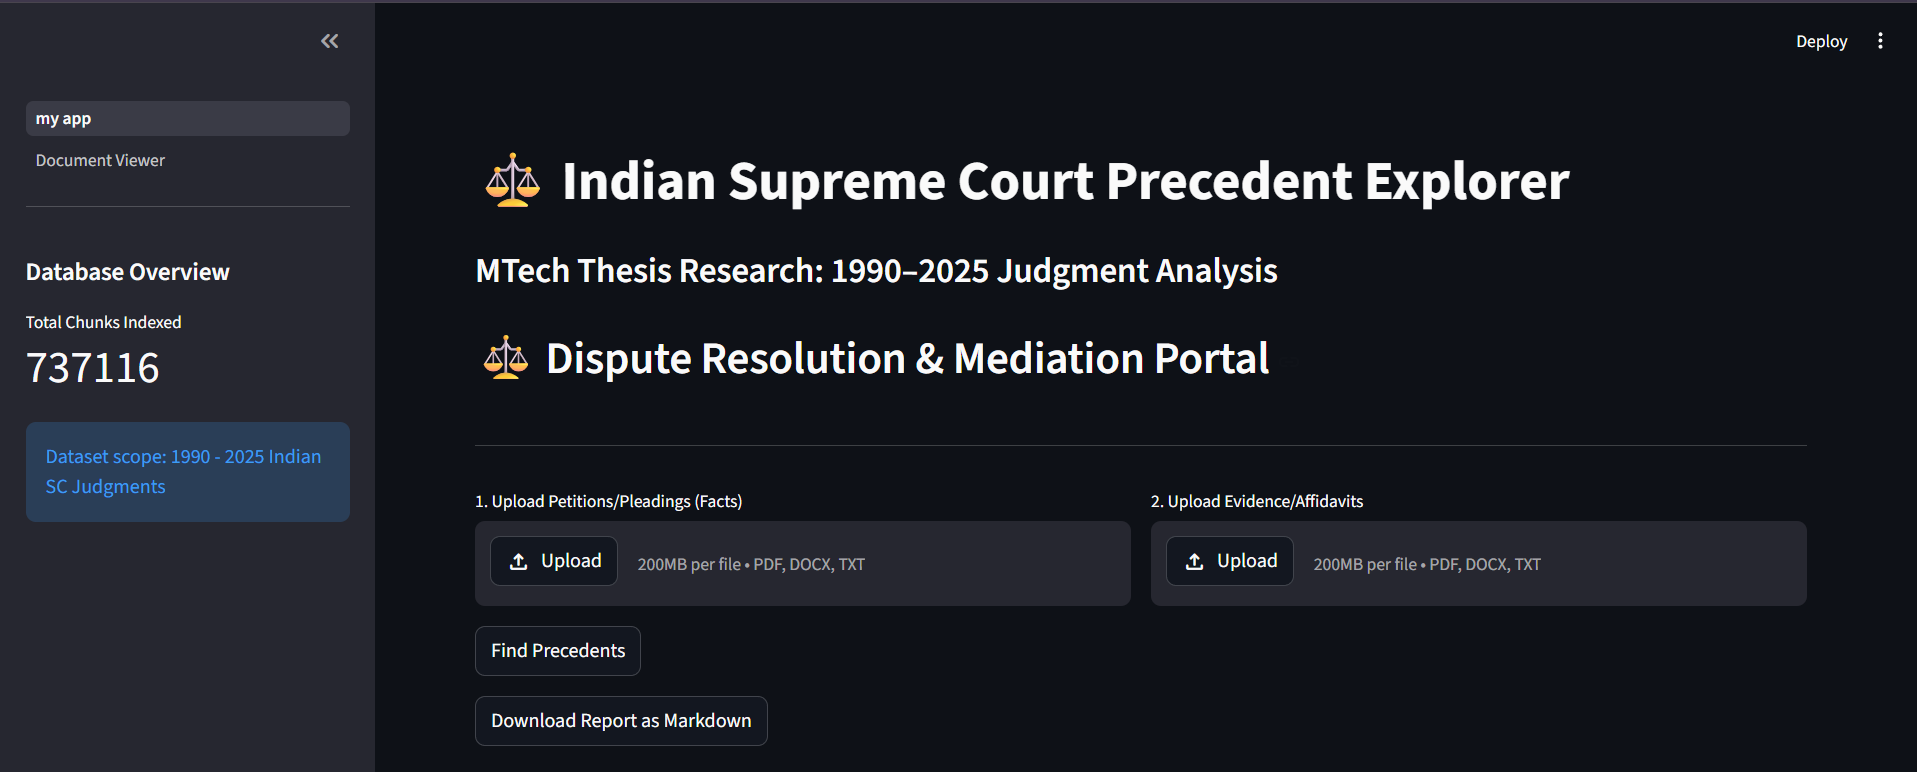
\includegraphics[width=0.8\textwidth]{figs/system_ss/0.png}
	\caption{Streamlit UI: Document upload interface, vector DB has ~700k Indexed chunks.}
	\label{fig:ui_upload}
\end{figure}

% Figure for Summary Output
\begin{figure}[htbp]
	\centering
	\captionsetup{justification=centering}
	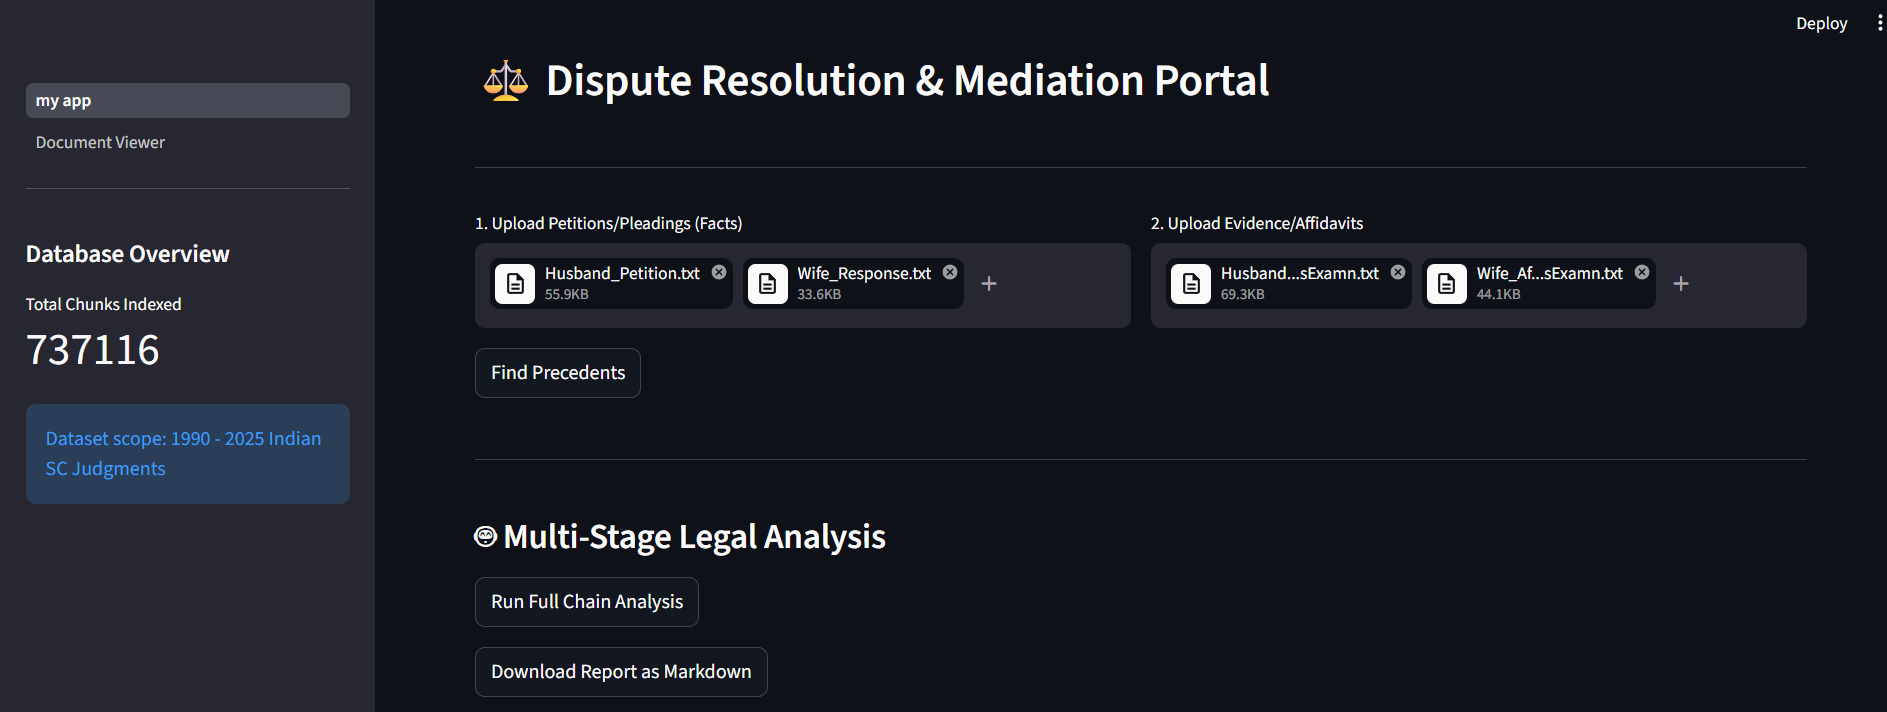
\includegraphics[width=0.8\textwidth]{figs/system_ss/1.png}
	\caption{UI to upload petition and evidence documents from both Petitioner and Respondent.}
	\label{fig:gemini_output}
\end{figure}


\begin{figure}[htbp]
	\centering
	\captionsetup{justification=centering}
	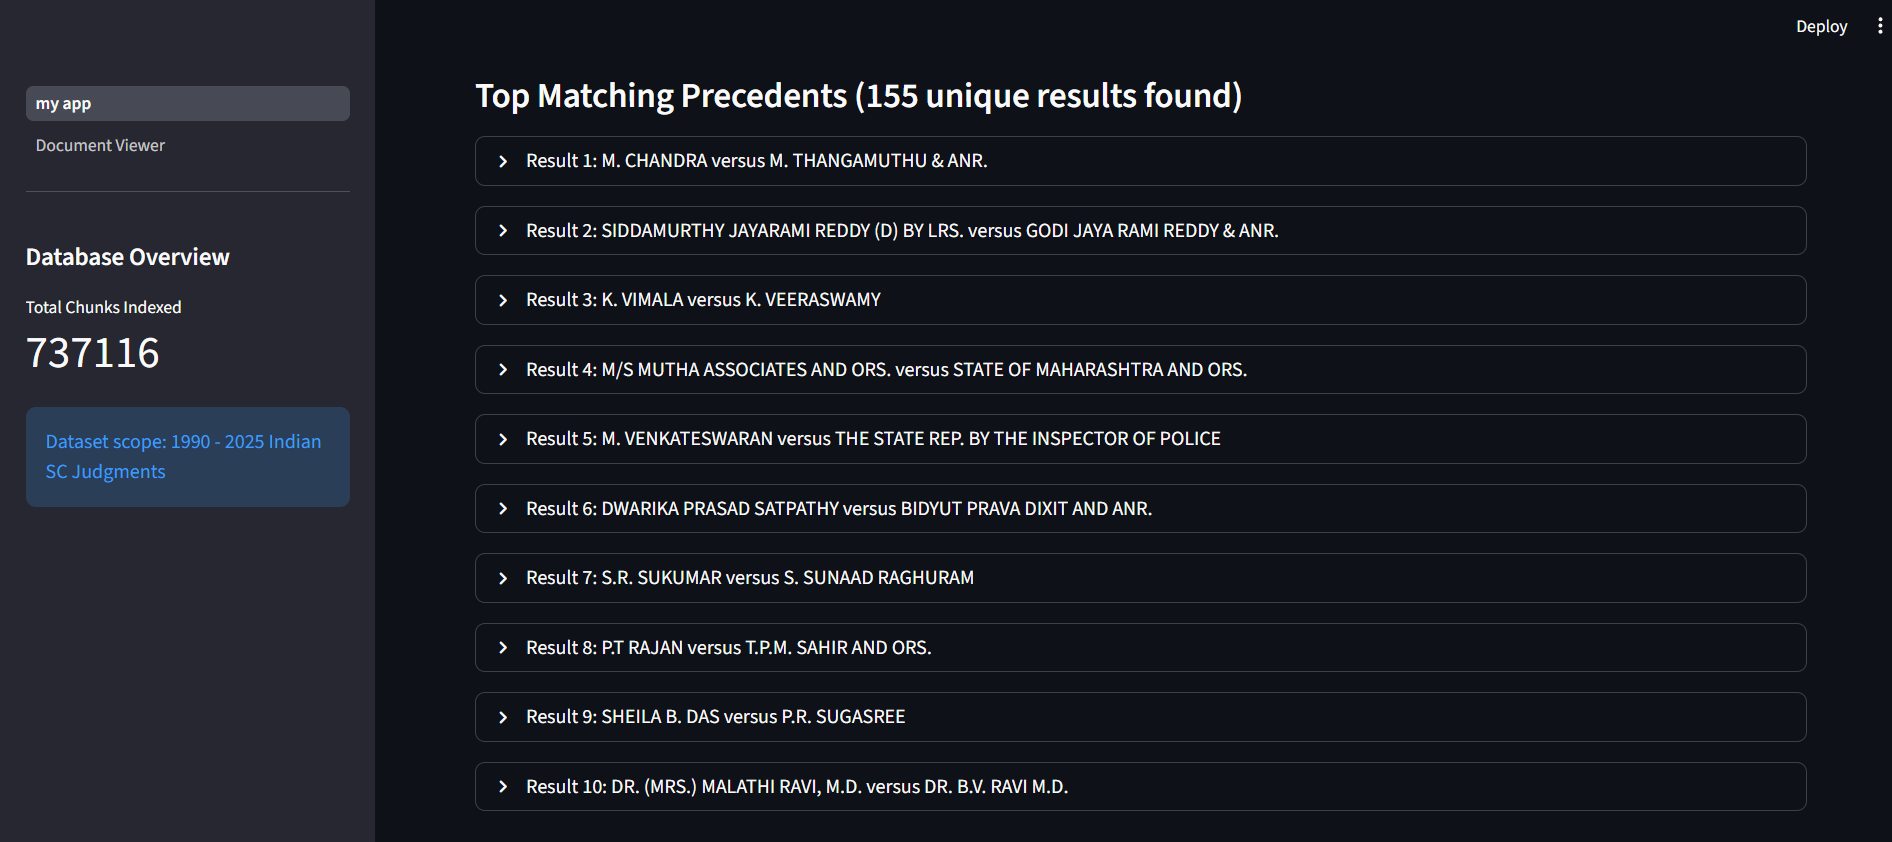
\includegraphics[width=0.8\textwidth]{figs/system_ss/2.png}
	\caption{Top 10 precedents displayed, total precedents found: 155.}
	\label{fig:gemini_output}
\end{figure}


\begin{figure}[htbp]
	\centering
	\captionsetup{justification=centering}
	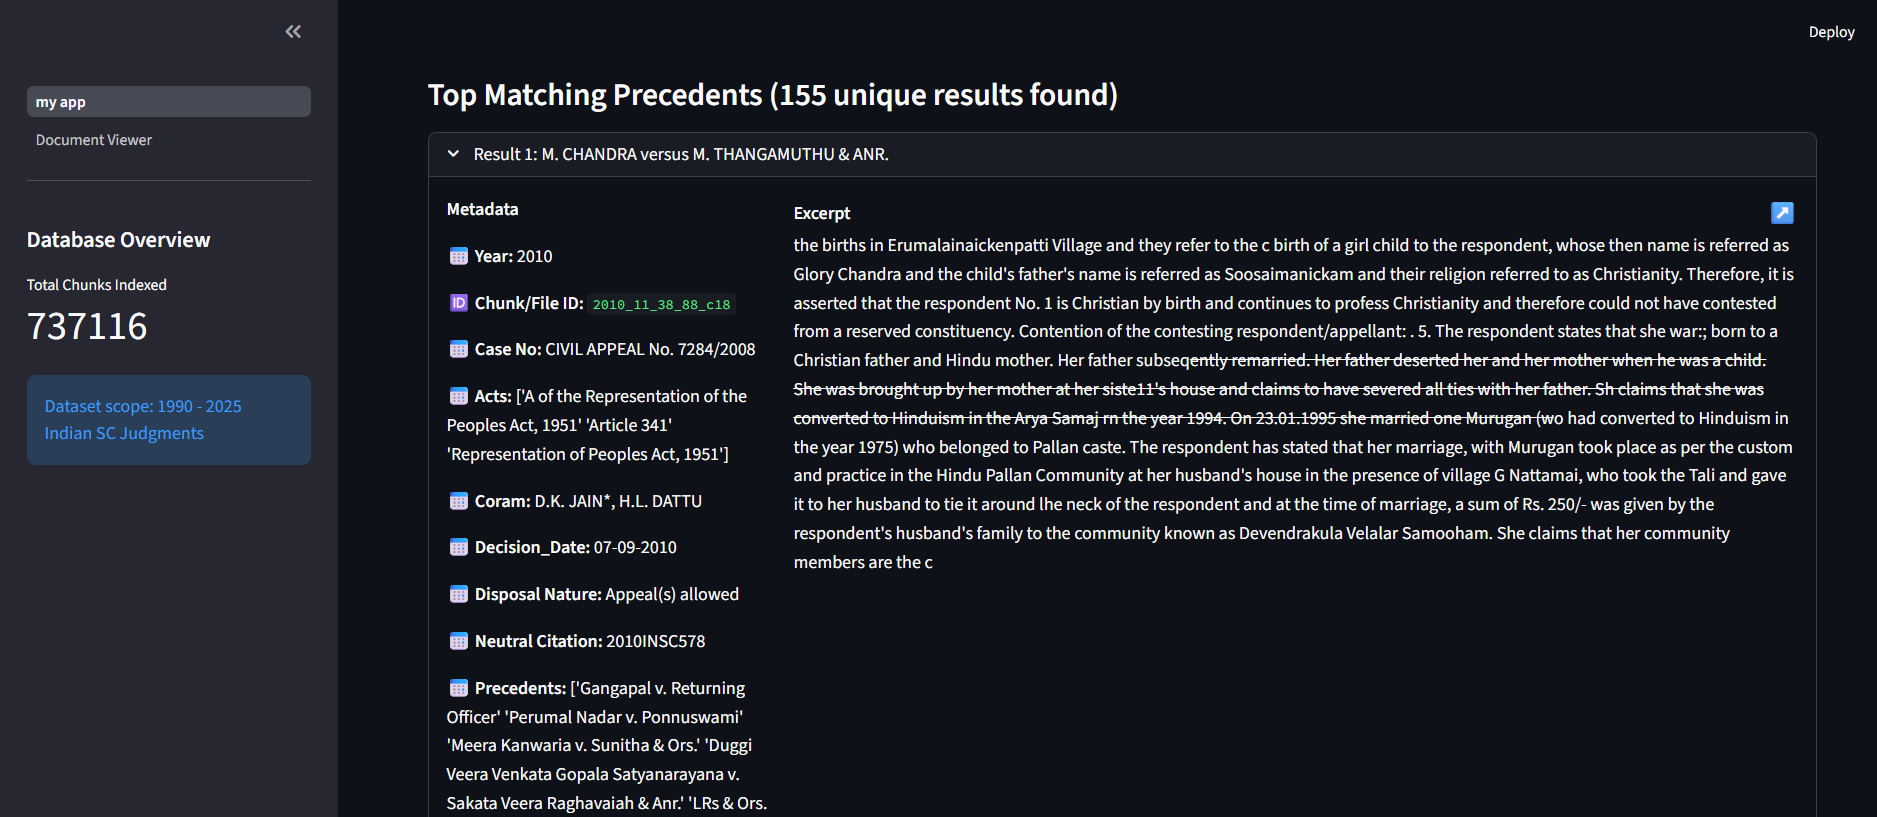
\includegraphics[width=0.8\textwidth]{figs/system_ss/3.png}
	\caption{View Precedent metadata.}
	\label{fig:gemini_output}
\end{figure}


\begin{figure}[htbp]
	\centering
	\captionsetup{justification=centering}
	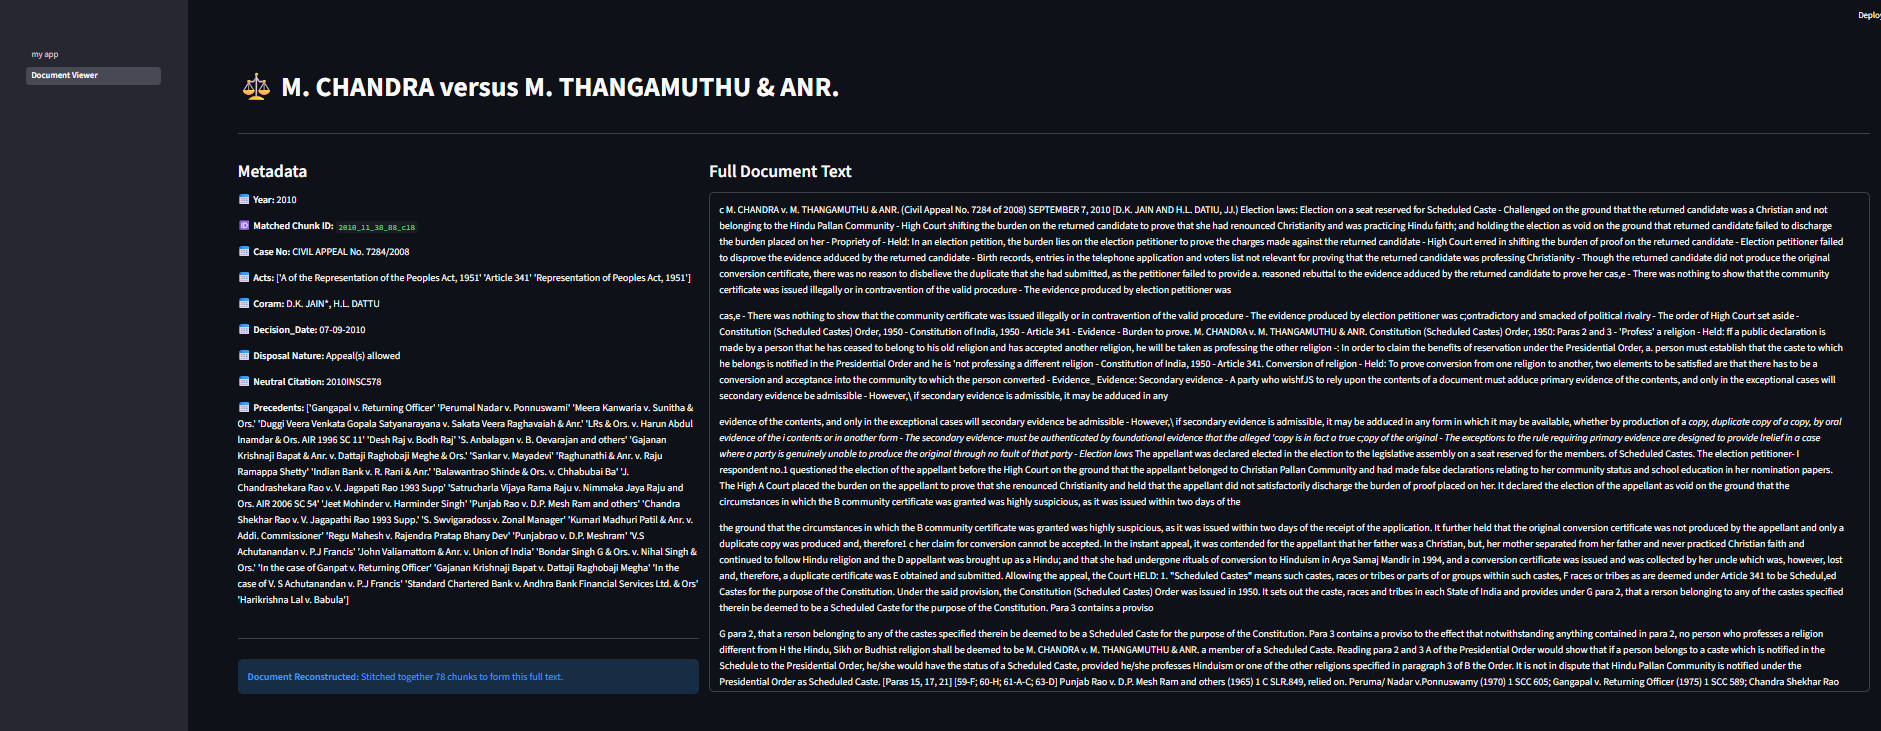
\includegraphics[width=0.8\textwidth]{figs/system_ss/3.5.png}
	\caption{View complete retrieved precedent details in separate tab.}
	\label{fig:gemini_output}
\end{figure}

\begin{figure}[htbp]
	\centering
	\captionsetup{justification=centering}
	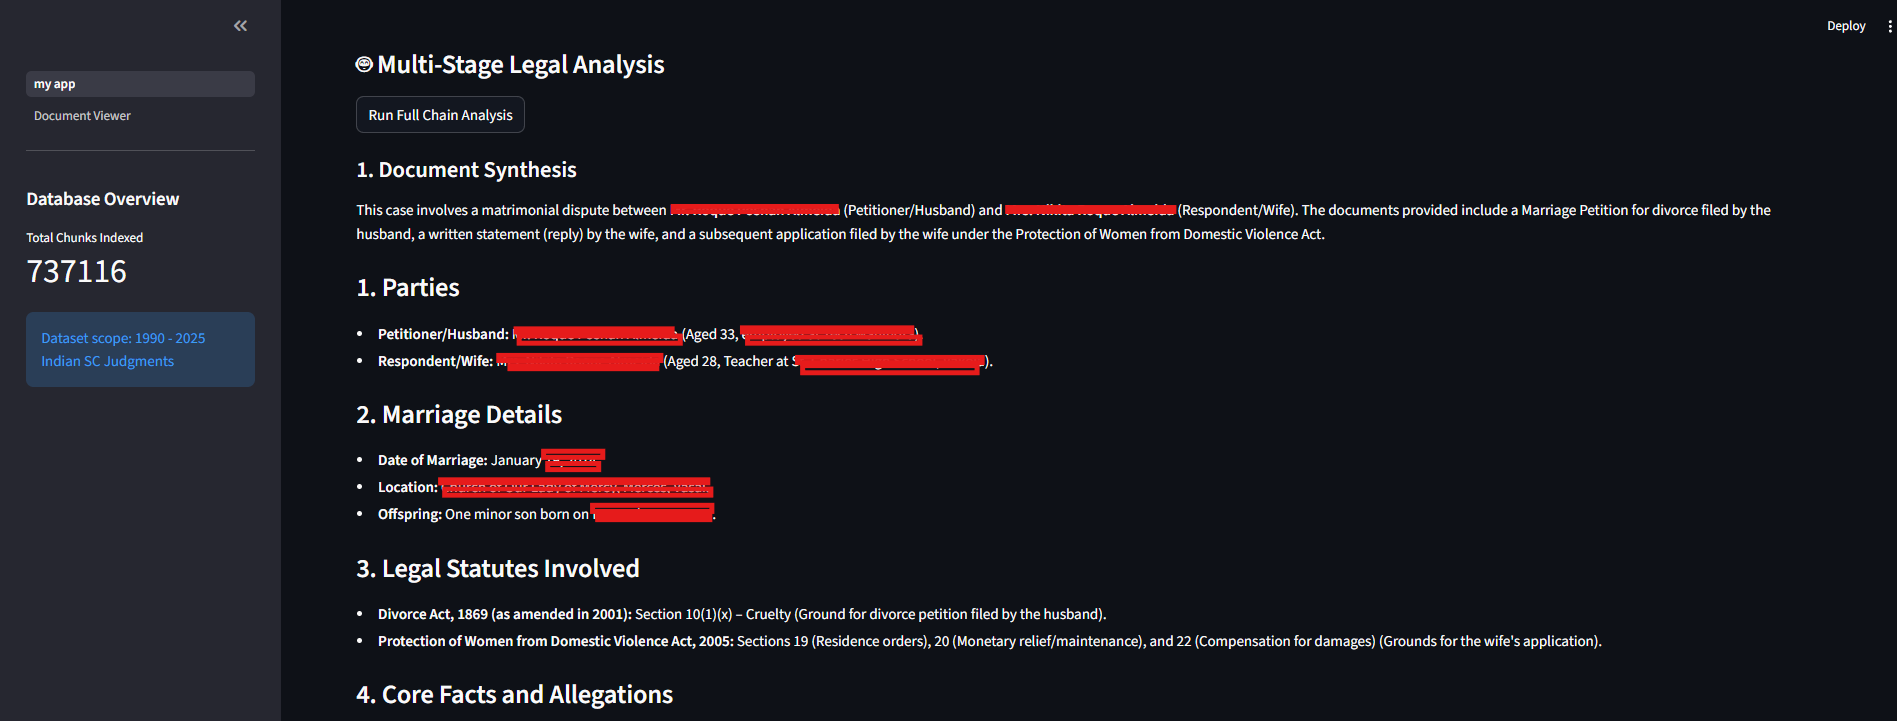
\includegraphics[width=0.8\textwidth]{figs/system_ss/4.png}
	\caption{Initial Document Synthesis Part 1.}
	\label{fig:gemini_output}
\end{figure}


\begin{figure}[htbp]
	\centering
	\captionsetup{justification=centering}
	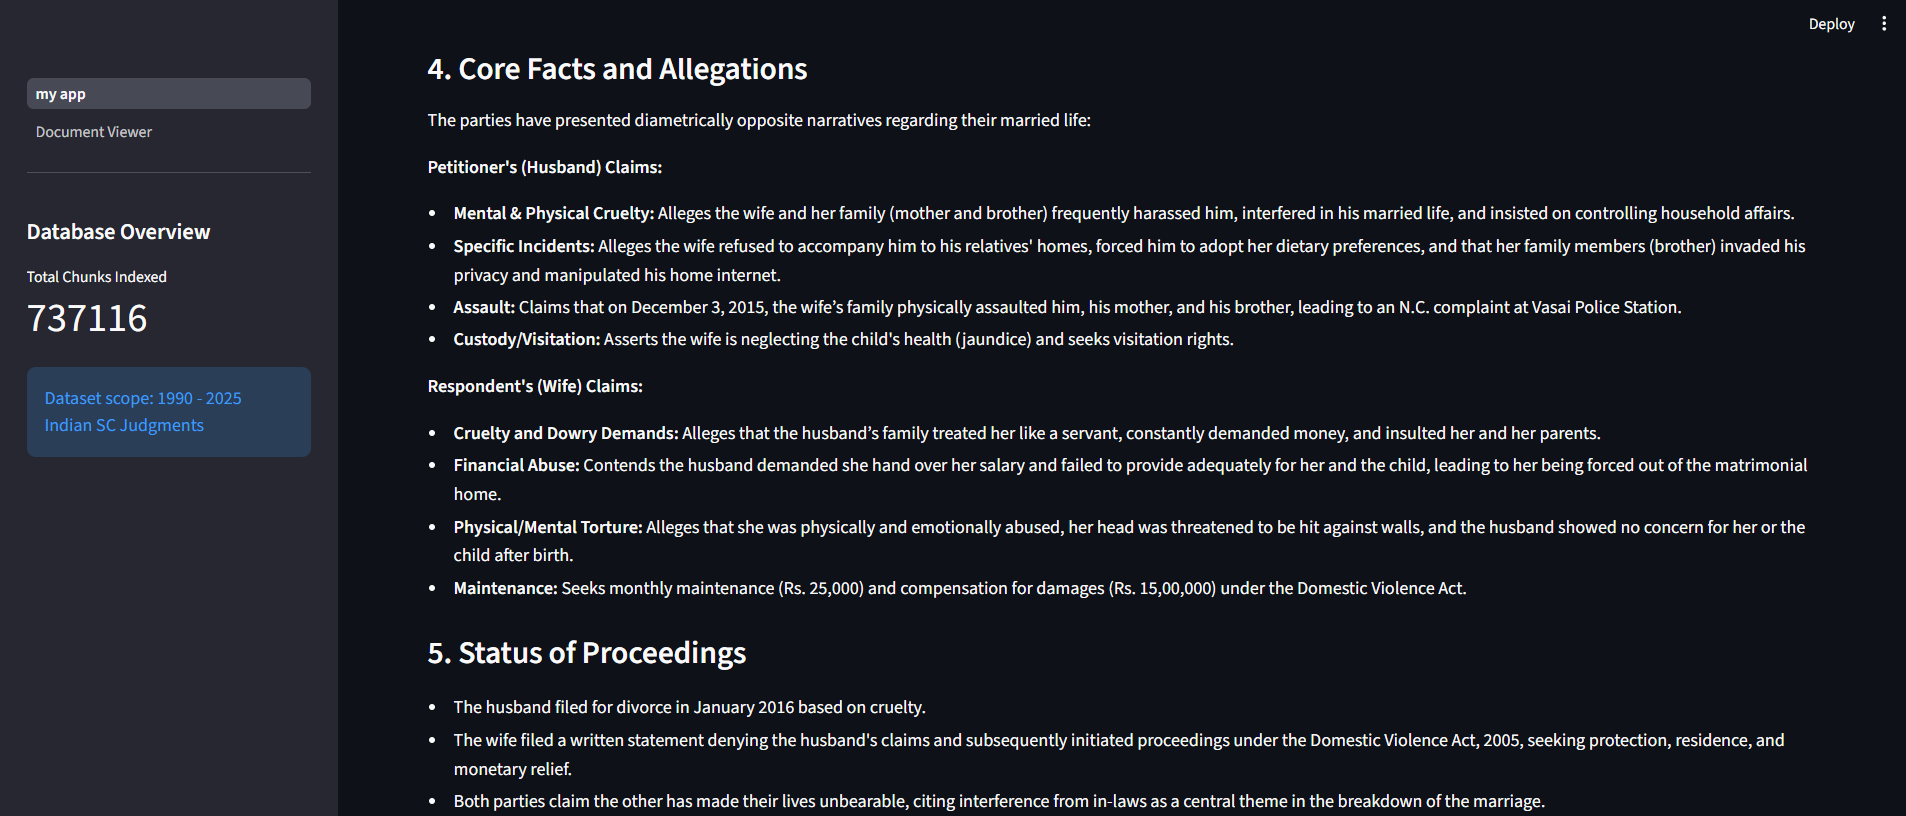
\includegraphics[width=0.8\textwidth]{figs/system_ss/5.png}
	\caption{Initial Document Synthesis Part 2.}
	\label{fig:gemini_output}
\end{figure}


\begin{figure}[htbp]
	\centering
	\captionsetup{justification=centering}
	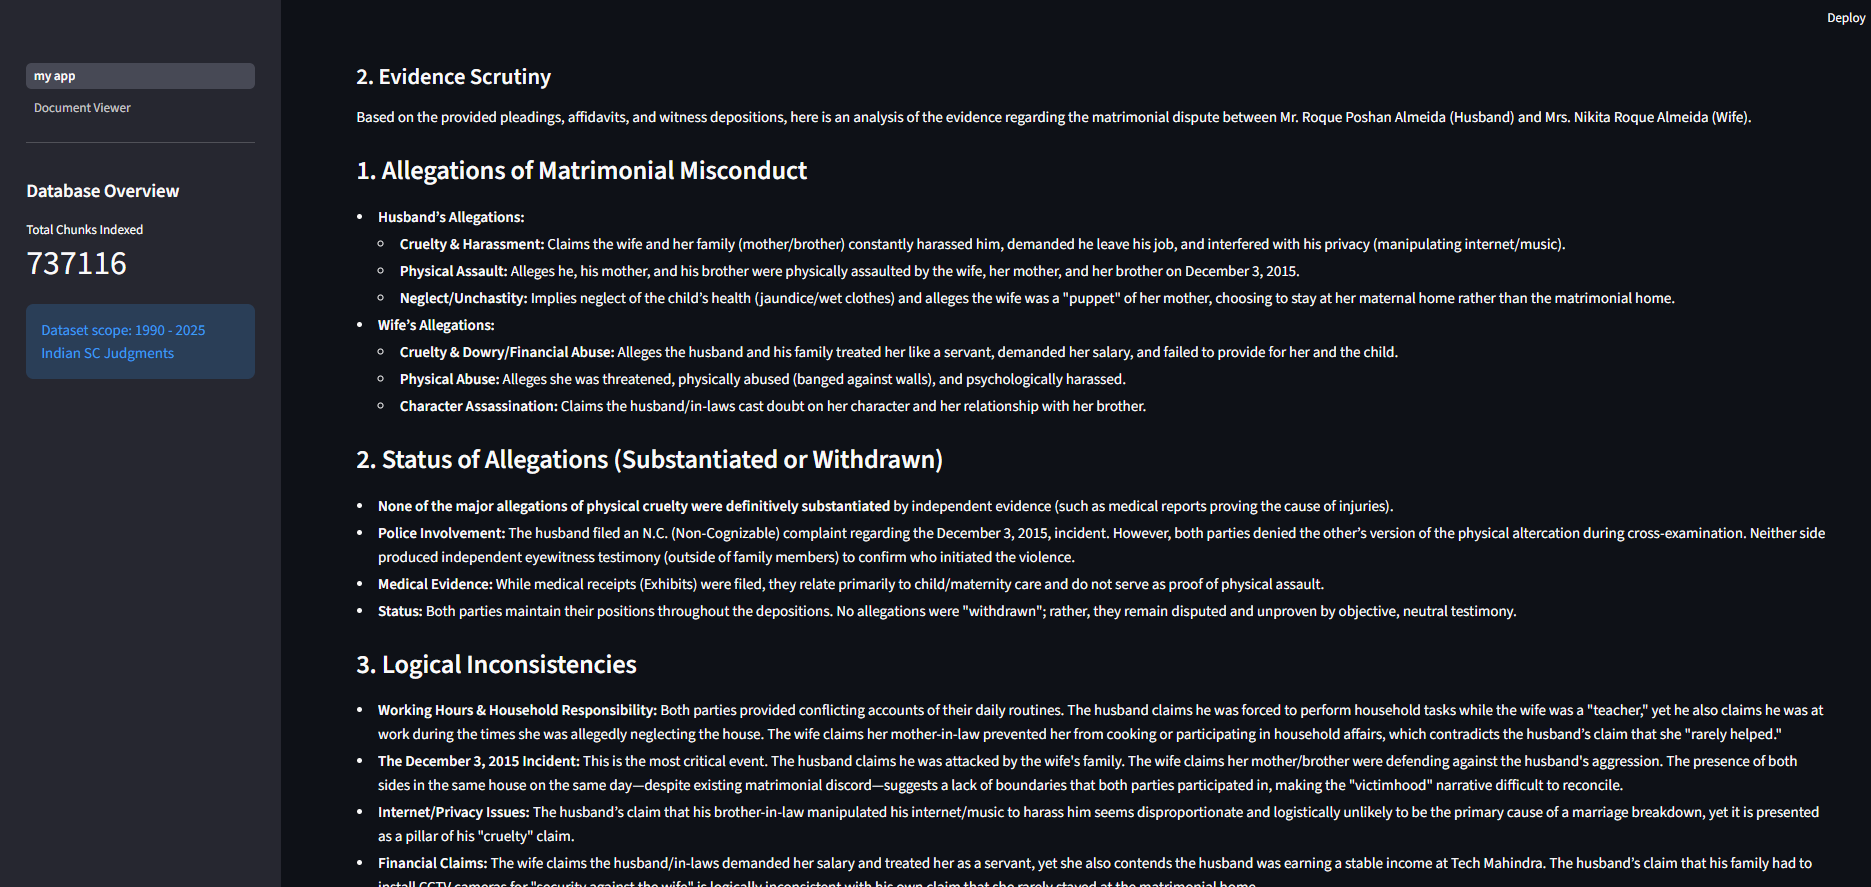
\includegraphics[width=0.8\textwidth]{figs/system_ss/6.png}
	\caption{Evidence Scrutinization Part 1.}
	\label{fig:gemini_output}
\end{figure}




\begin{figure}[htbp]
	\centering
	\captionsetup{justification=centering}
	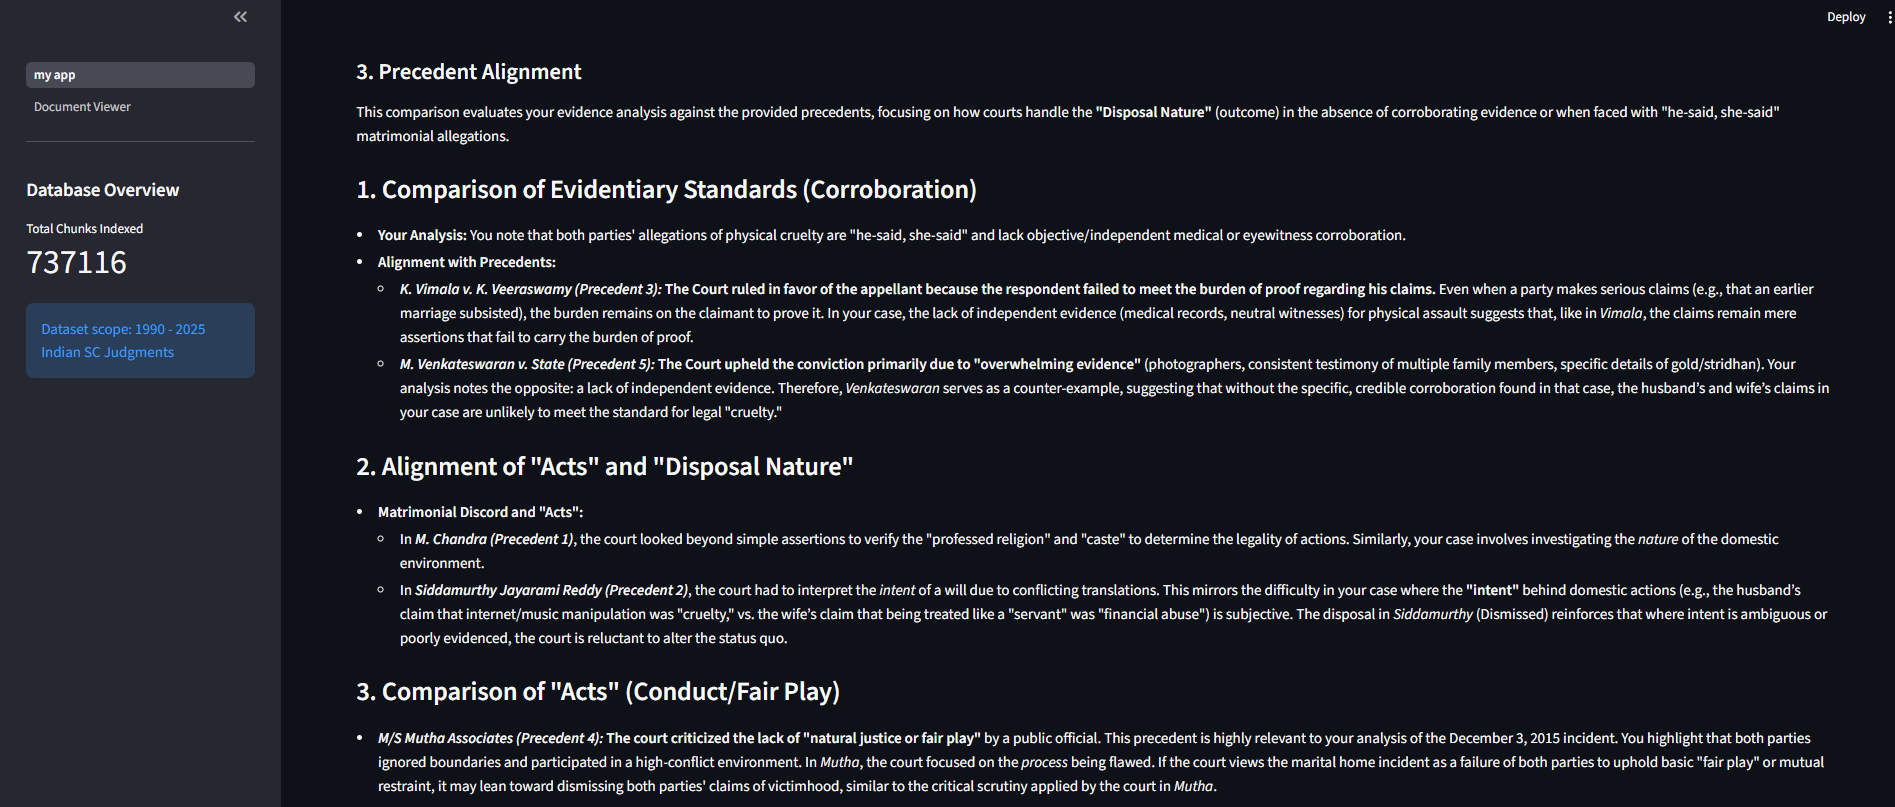
\includegraphics[width=0.8\textwidth]{figs/system_ss/7.png}
	\caption{Evidence Scrutinization Part 2: Precedent Alignment.}
	\label{fig:gemini_output}
\end{figure}


\begin{figure}[htbp]
	\centering
	\captionsetup{justification=centering}
	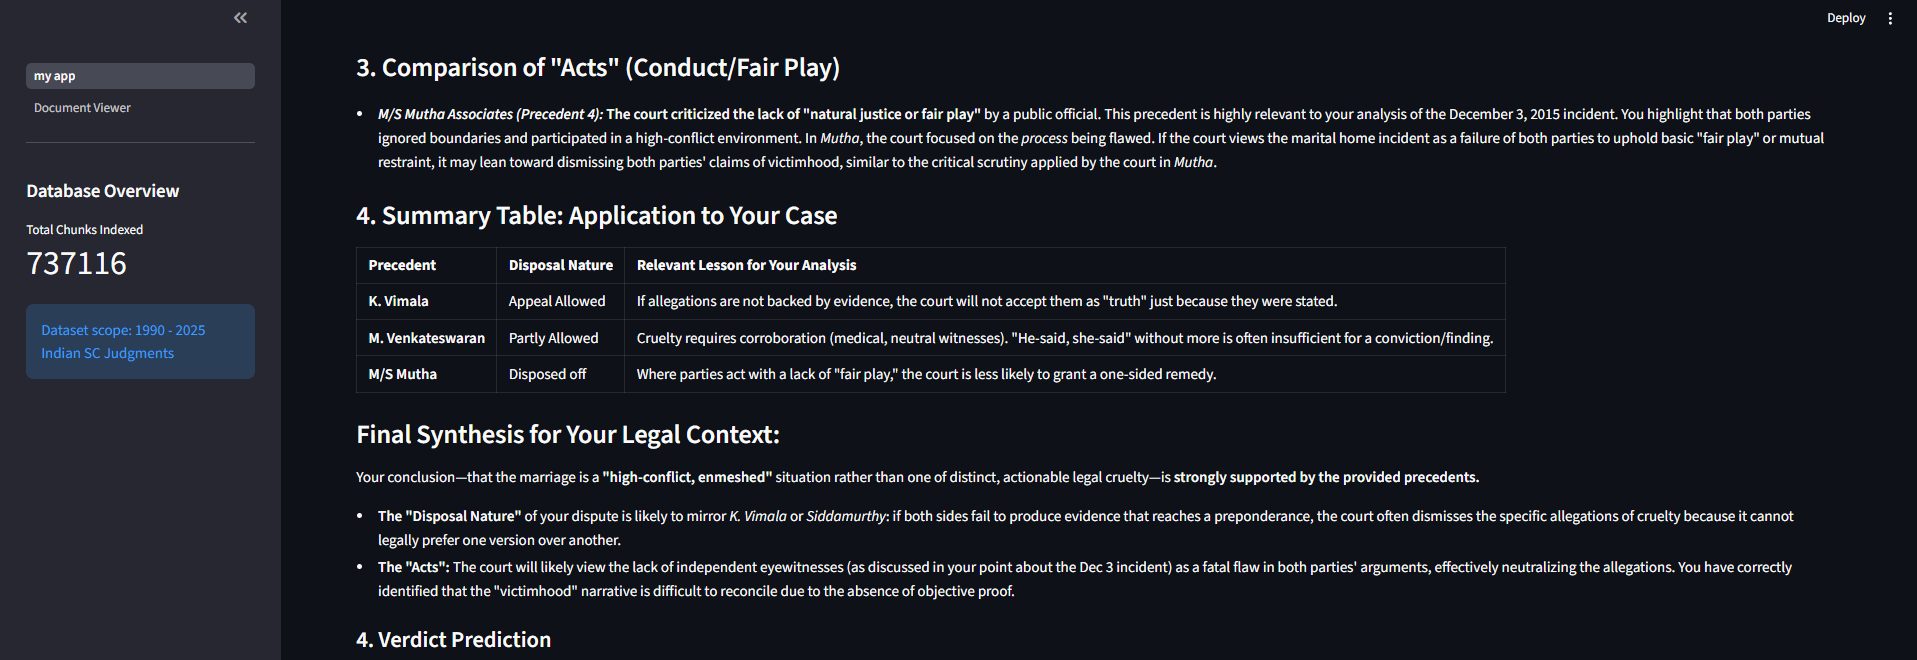
\includegraphics[width=0.8\textwidth]{figs/system_ss/8.png}
	\caption{Final Synthesis.}
	\label{fig:gemini_output}
\end{figure}


\begin{figure}[htbp]
	\centering
	\captionsetup{justification=centering}
	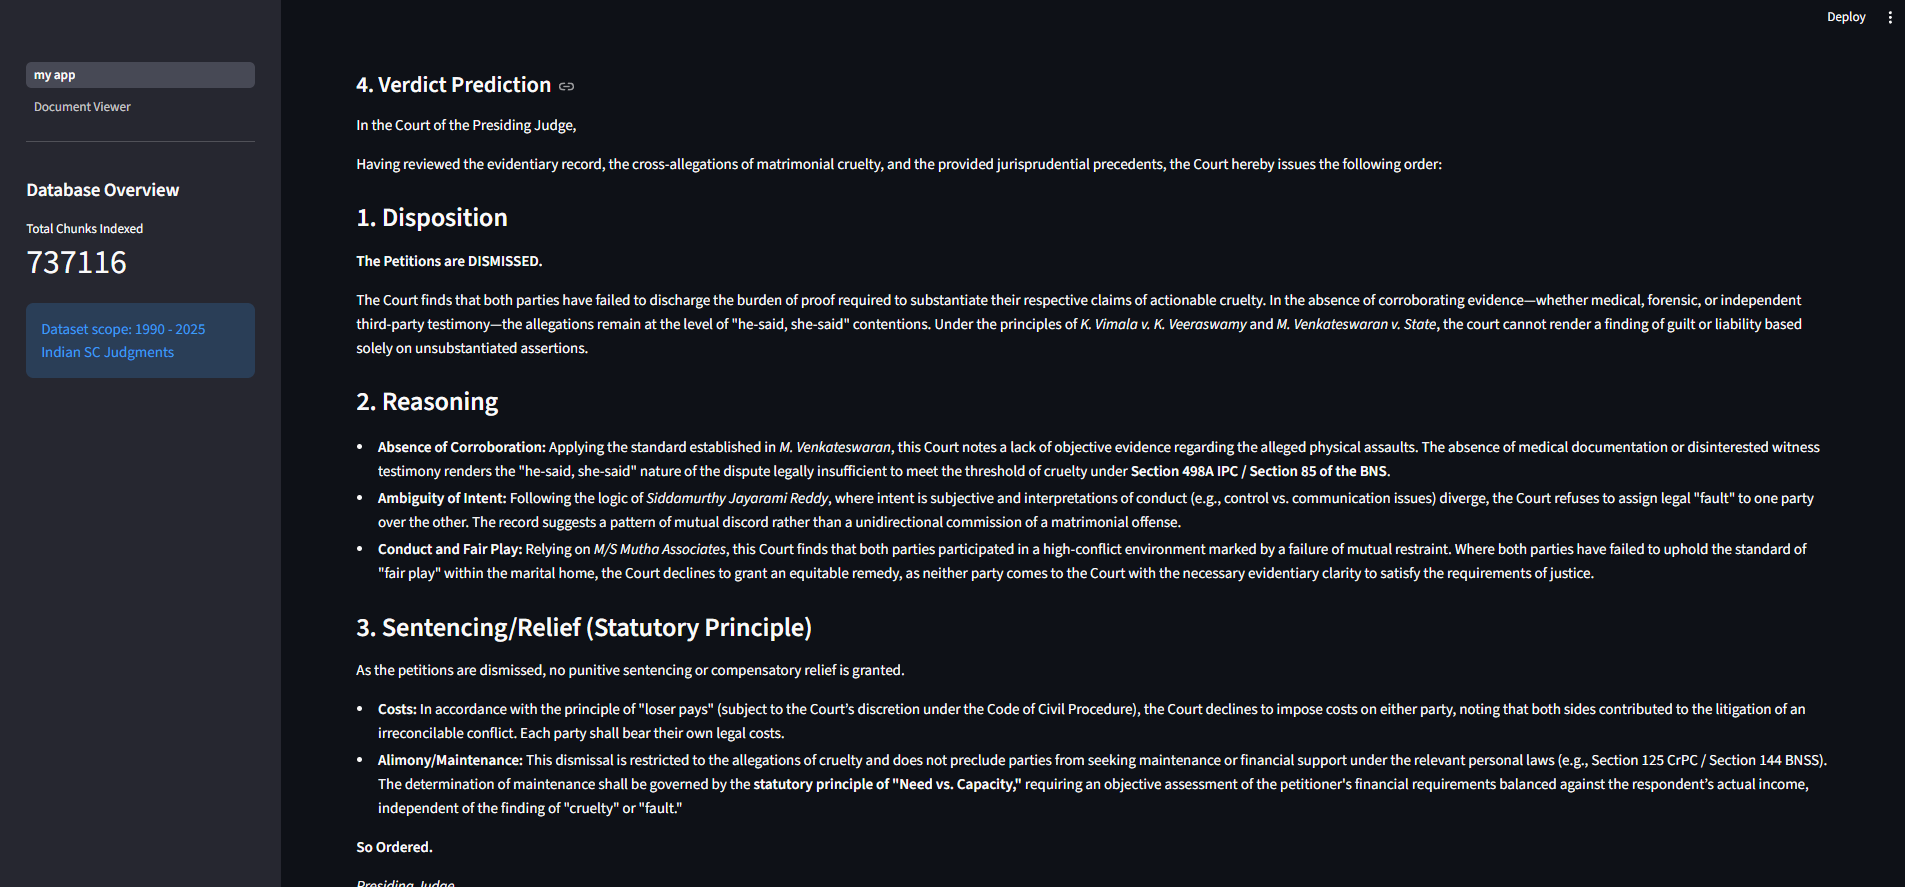
\includegraphics[width=0.8\textwidth]{figs/system_ss/9.png}
	\caption{Prediction of Verdict, Sentence \& Relief.}
	\label{fig:gemini_output}
\end{figure}


\begin{figure}[htbp]
	\centering
	\captionsetup{justification=centering}
	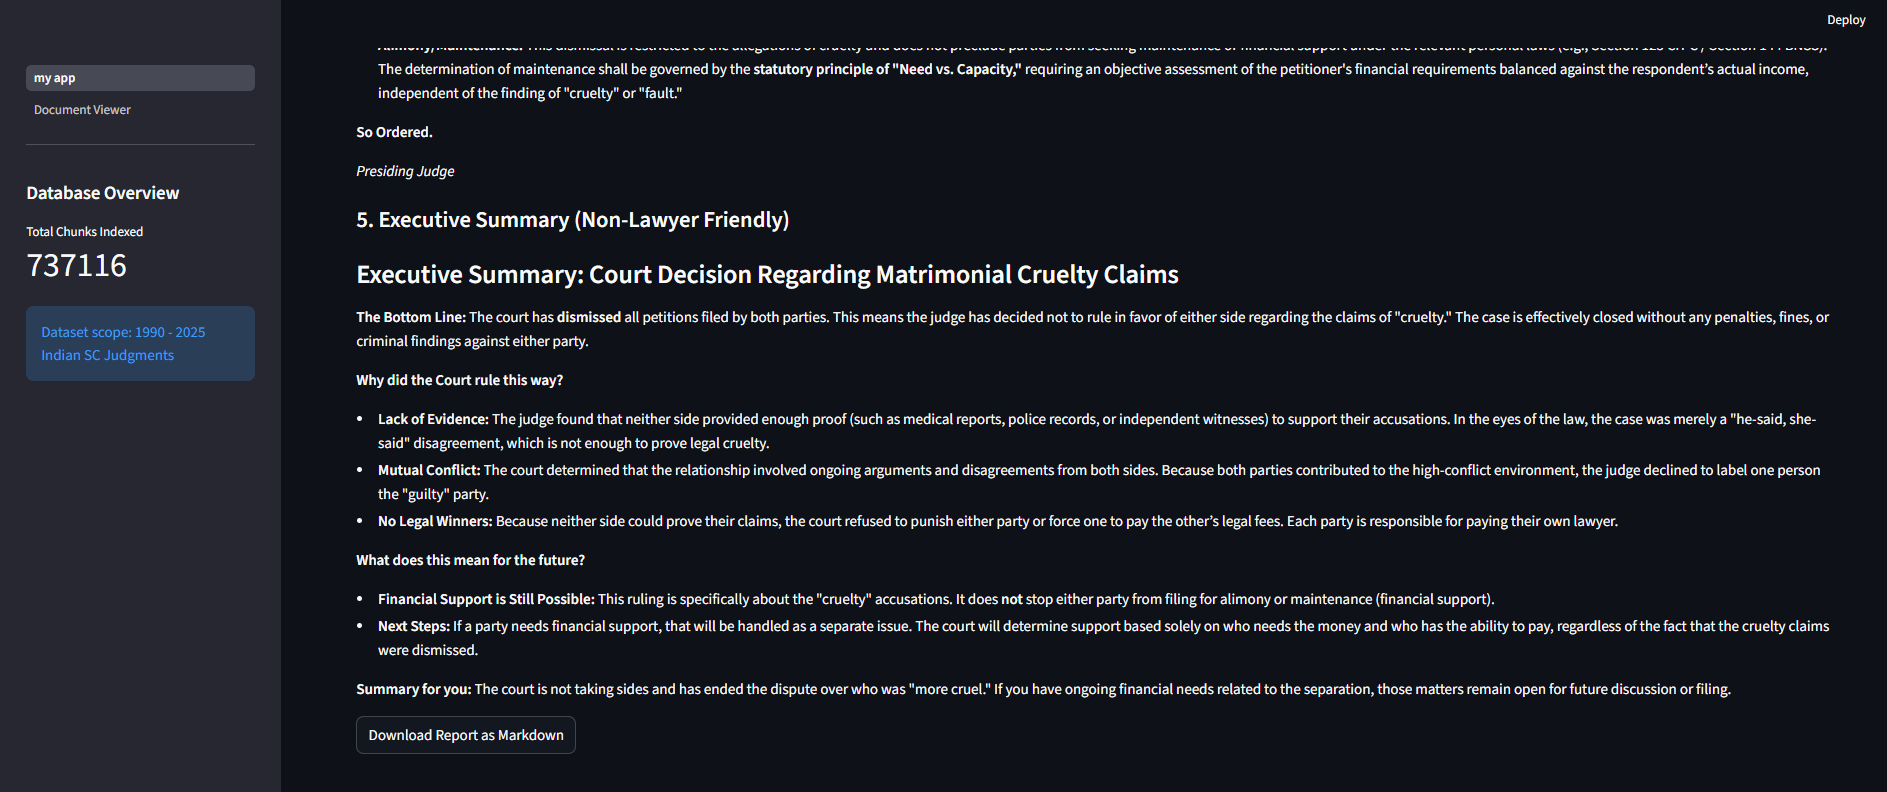
\includegraphics[width=0.8\textwidth]{figs/system_ss/10.png}
	\caption{Output Summarization.}
	\label{fig:gemini_output}
\end{figure}








